
\documentclass{beamer}

\usepackage{hyperref}
\usetheme{Singapore}
\usecolortheme[RGB={0, 32, 91}]{structure}  % Rice blue
\setbeamertemplate{navigation symbols}{\insertframenumber}

\definecolor{riceblue}{rgb}{0.000, 0.125, 0.357}
\definecolor{ricegray}{rgb}{0.486, 0.494, 0.498}
\definecolor{ricerichblue}{rgb}{0.039, 0.314, 0.620}

\title{Pitch trajectory density estimation \\ for predicting future outcomes}
\author{\color{ricerichblue} Scott Powers and Vicente Iglesias}
\date{Saberseminar 2023}

\begin{document}

  \begin{frame}
    \maketitle
    \vfill
    \hfill
    
\includegraphics[width = 0.5\textwidth]{images/rice_smgt.png}
  \end{frame}

  \begin{frame}{Pitch Modeling}
    \centering
    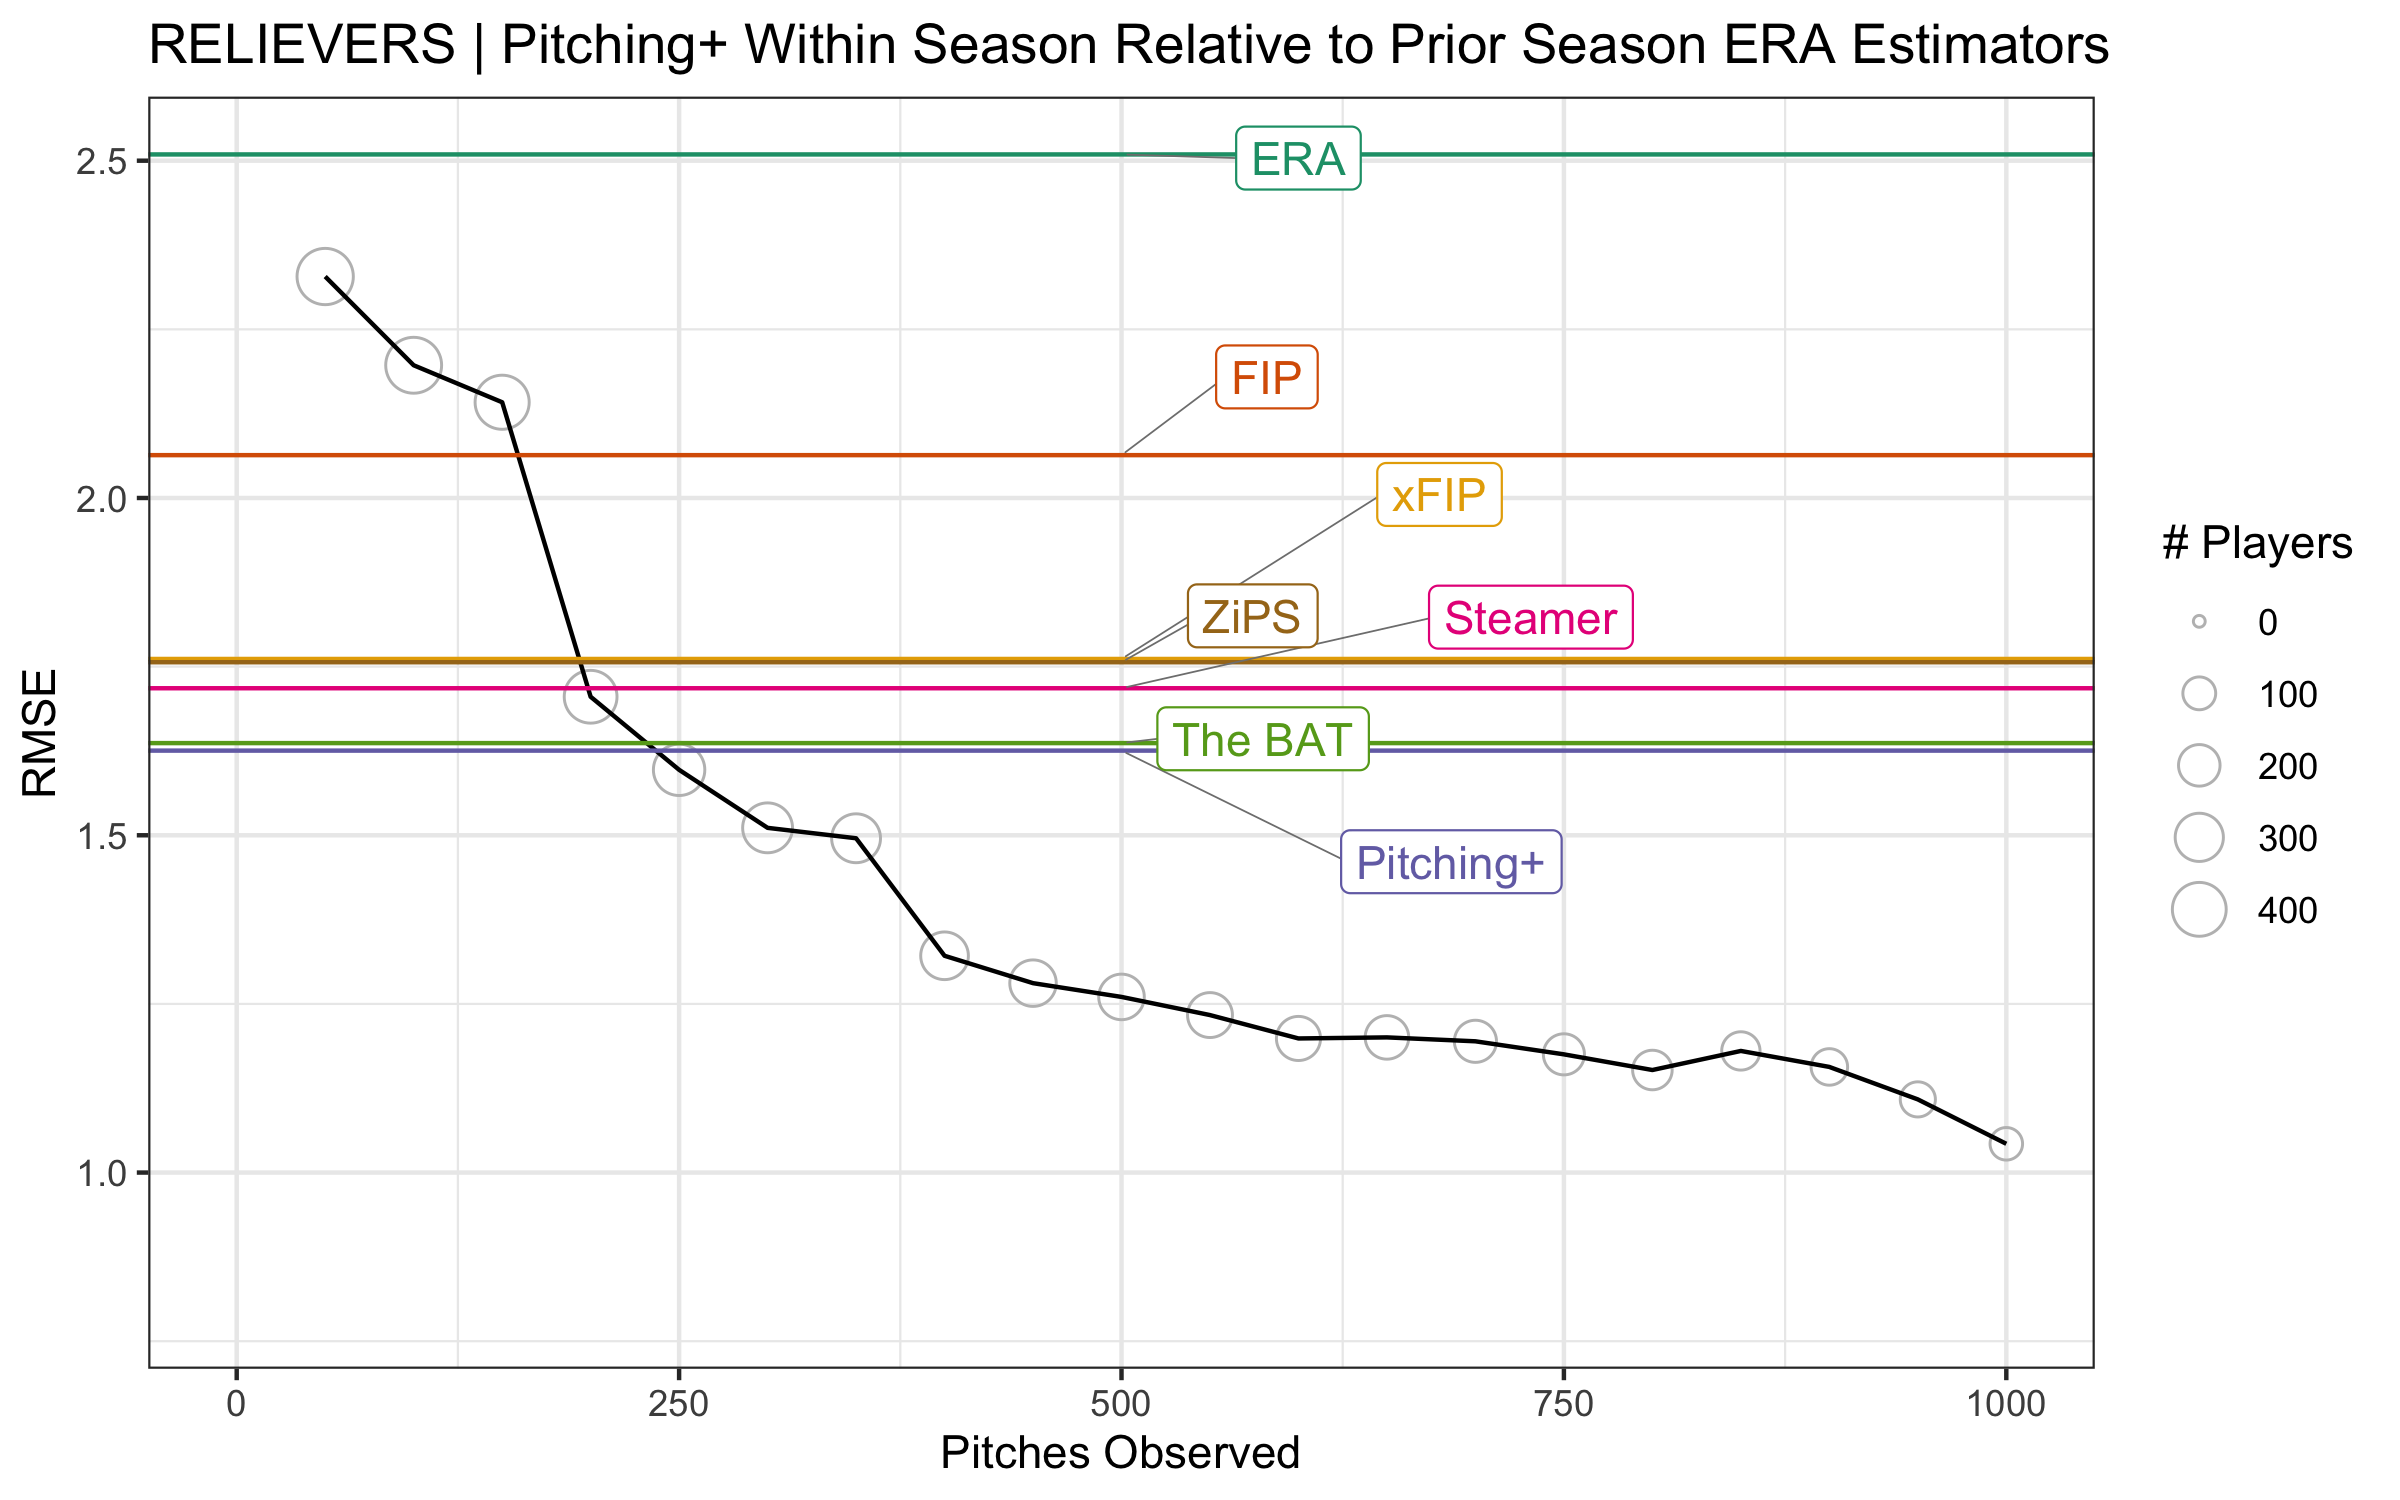
\includegraphics[width = \textwidth]{images/pitching_plus.png}\\
    \color{ricegray} \scriptsize https://library.fangraphs.com/pitching/stuff-location-and-pitching-primer/
  \end{frame}

  \begin{frame}{The Conundrum}
    \begin{columns}
      \begin{column}{0.5\textwidth}
        \centering
        $\mbox{Variable Importance}^1$\\
        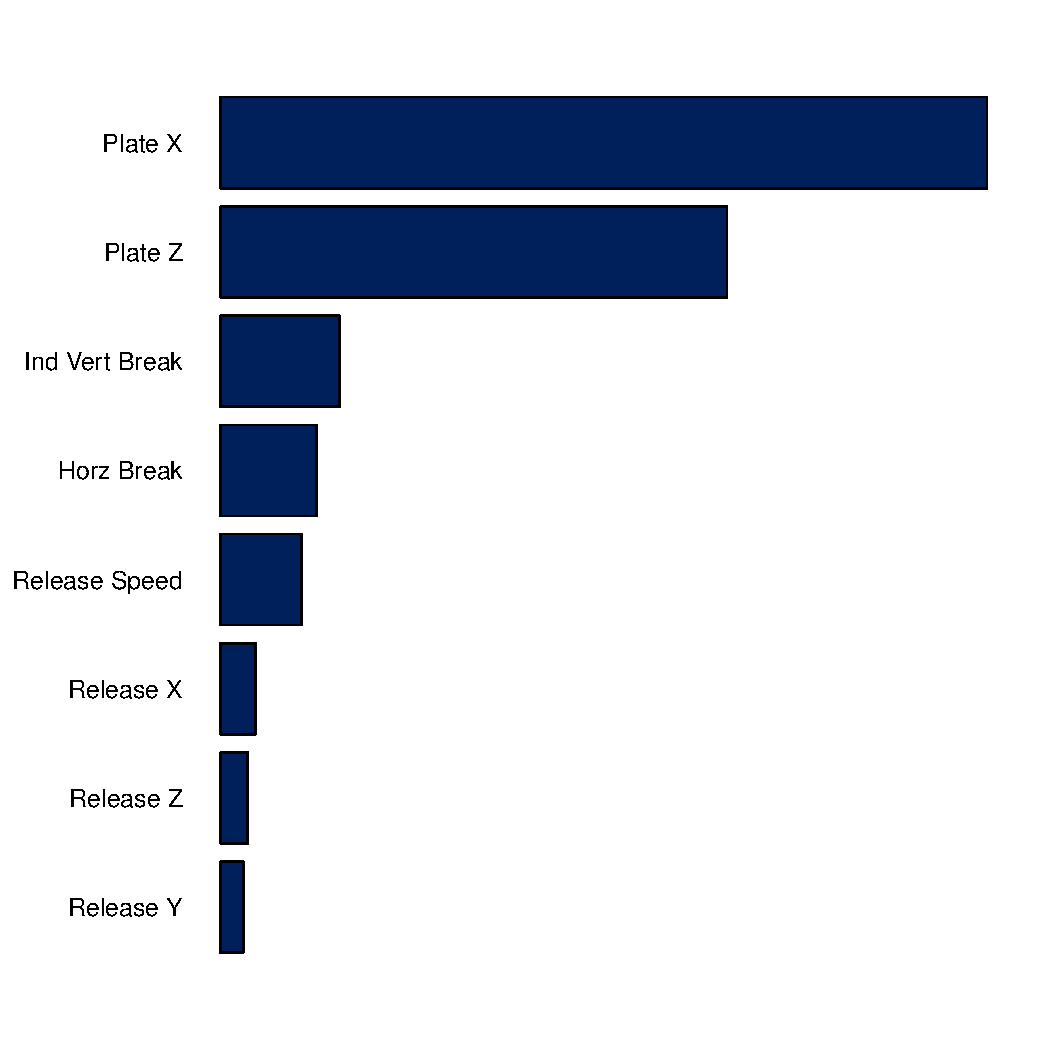
\includegraphics[width = \textwidth]{images/feature_importance.pdf}
      \end{column}
      \begin{column}{0.5\textwidth}
        \centering
        $\mbox{Variable Reliability}^2$\\
        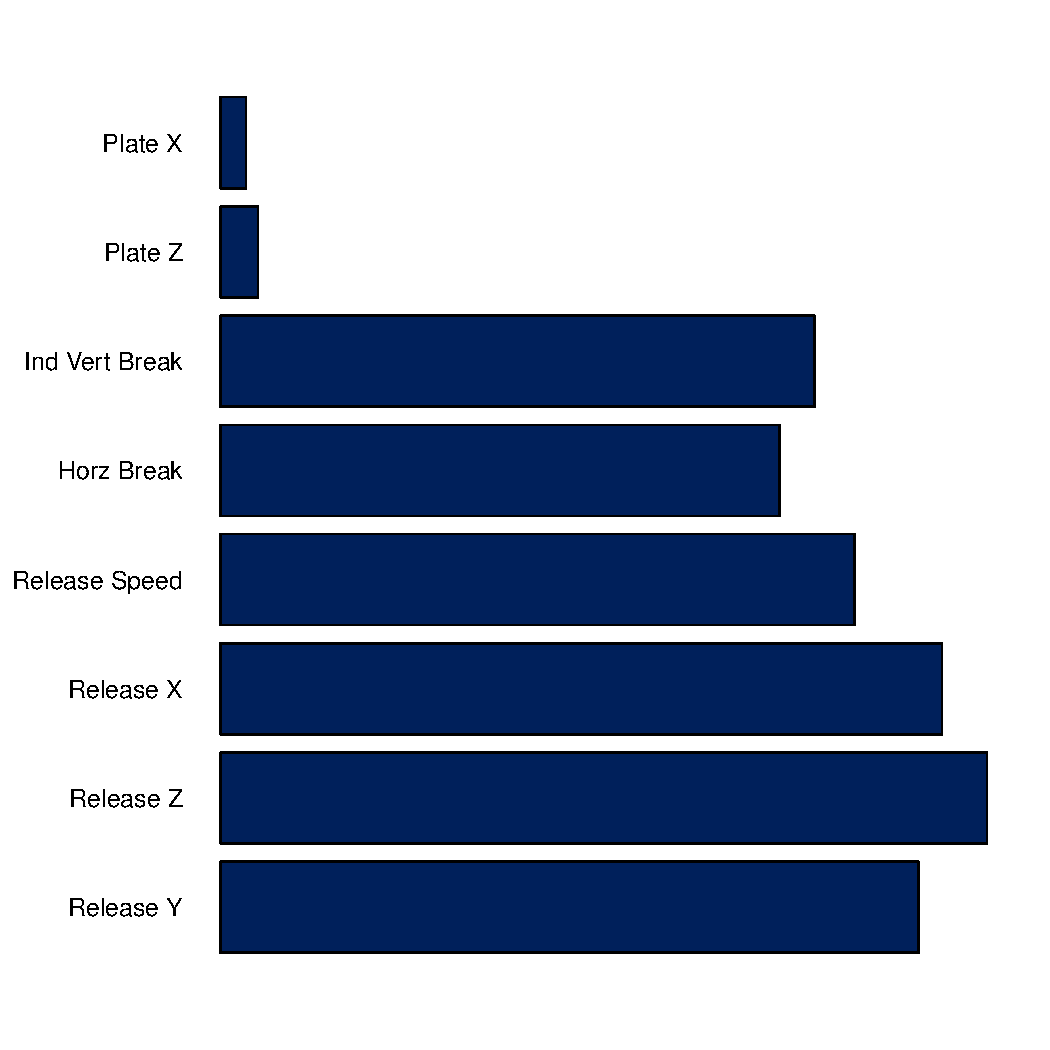
\includegraphics[width = \textwidth]{images/feature_reliability.pdf}
      \end{column}
    \end{columns}
    \scriptsize \color{ricegray}
    \vfill
    ${}^1$ fractional contribution of each feature's splits to gradient boosting pitch model\\
    ${}^2$ (between-pitcher variance) / (total variance); varies by pitch type (here: RHB FB)
  \end{frame}

  \begin{frame}{An Example}
    \begin{columns}
      \begin{column}{0.2\textwidth}
        \centering
        Pitch A\\
        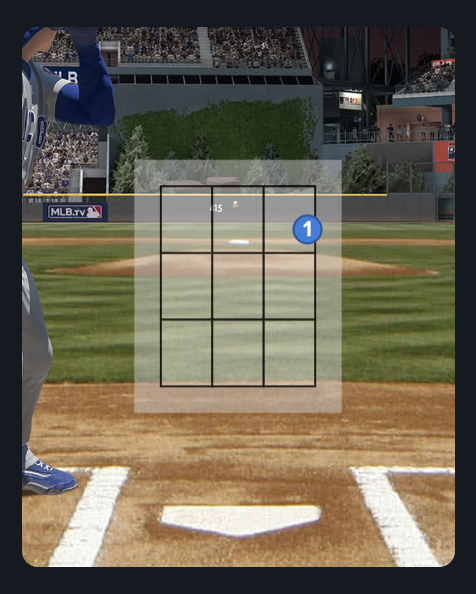
\includegraphics[width = \textwidth]{images/pitch_on_edge}
      \end{column}
      \begin{column}{0.8\textwidth}
        \begin{itemize}
          \item 91 mph fastball
          \item 15 inches rise
          \item located on the edge of the zone
          \item 68\% called strike, 11\% foul, 8\% ball in play,\\
            8\% called ball, 5\% swinging strike ($-0.04$ runs)
        \end{itemize}
      \end{column}
    \end{columns}
    ~\\
    ~\\
    \begin{columns}
      \begin{column}{0.2\textwidth}
        \centering
        Pitch B\\
        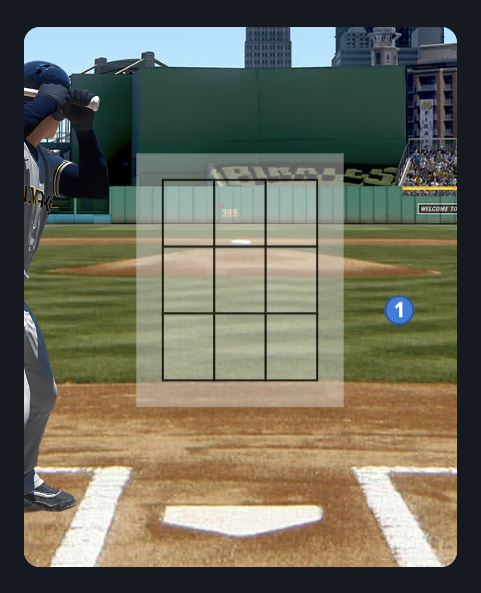
\includegraphics[width = \textwidth]{images/pitch_outside}
      \end{column}
      \begin{column}{0.8\textwidth}
        \begin{itemize}
          \item 98 mph fastball
          \item 20 inches rise
          \item located a foot off of the plate
          \item 99.6\% called ball ($+0.04$ runs)
        \end{itemize}
      \end{column}
    \end{columns}
  \end{frame}

  \begin{frame}{Two Sources of Noise}
    \begin{enumerate}
      \item Random variation in the outcome given the pitch trajectory
      \begin{itemize}
        \item This is addressed by Pitching+, PitchingBot, etc.
      \end{itemize}
      ~\\
      \item Random variation in the pitch trajectory itself
      \begin{itemize}
        \item This is NOT addressed by Pitching+, PitchingBot, etc.
      \end{itemize}
    \end{enumerate}
  \end{frame}

  \begin{frame}{The Approach}
    \begin{enumerate}
      \item Fit a model to predict pitch outcome given its trajectory
      \begin{itemize}
        \item We use gradient boosting, not the focus today
      \end{itemize}
      ~\\
      \item Estimate the probability distribution over pitch trajectories
      \begin{itemize}
        \item Depends on pitcher, batter side, count, etc.
      \end{itemize}
      ~\\
      \item Apply the model {\color{riceblue} 1.} to the distribution {\color{riceblue} 2.}
      \begin{itemize}
        \item As opposed to applying the model to the observed pitches
      \end{itemize}
    \end{enumerate}
  \end{frame}

  \begin{frame}{Bayesian Hierarchical Model}
    Within each pitch type:
    \begin{itemize}
      \item We model each pitch as multivariate normal in 9 dimensions
      \begin{itemize}
        \item x/y/z release point, x/y/z release velocity, x/y/z acceleration
      \end{itemize}
      \item Each pitcher has 81 parameters:
      \begin{itemize}
        \item $9 \times 4 = 36$ parameters for {\bf mean}
        \begin{itemize}
          \item Main effect plus interactions w/ balls, strikes, batter side
        \end{itemize}
        \item $9 \times 1 = 9$ parameters for {\bf variance}
        \item $\binom{9}{2} = 36$ parameters for {\bf correlation} between dimensions
      \end{itemize}
      \item Each (ball, strike, batter side) combo has 18 parameters:
      \begin{itemize}
        \item 9 parameters for mean, 9 parameters for variance
      \end{itemize}
      \item We find the maximum {\it a posteriori} (MAP) model fit using the \texttt{optimize} function (automatic differentiation) from cmdstanr
    \end{itemize}
  \end{frame}

  \begin{frame}{Dylan Cease's Slider vs RHB in 0-0 Counts}
    \begin{columns}
      \begin{column}{0.5\textwidth}
        \centering
        Predicted Break Chart\\
        \vspace{4mm}
        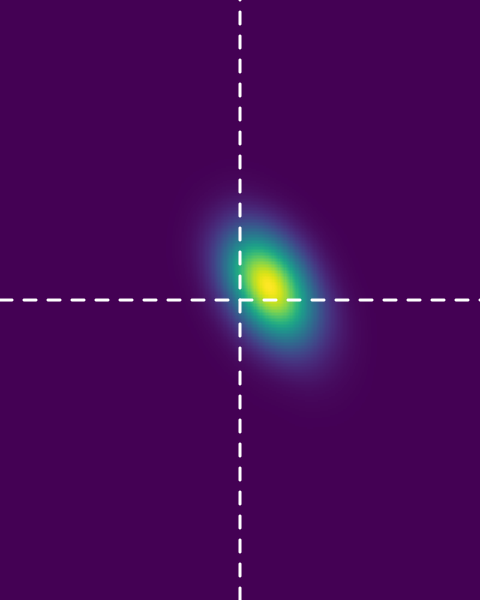
\includegraphics[width = 0.8\textwidth]{images/656302_SL_R_0_0_break.png}
      \end{column}
      \begin{column}{0.5\textwidth}
        \centering
        Predicted Plate Location\\
        \vspace{4mm}
        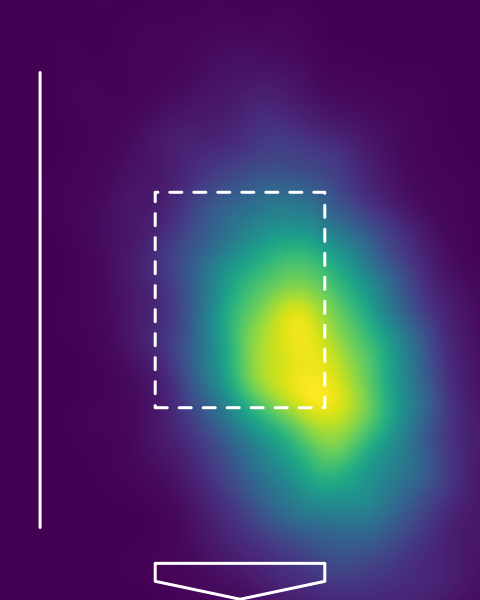
\includegraphics[width = 0.8\textwidth]{images/656302_SL_R_0_0_plate.png}
      \end{column}
    \end{columns}
    \vfill
    \centering \scriptsize {\color{ricerichblue}saberpowers}{\color{ricegray}.shinyapps.io/}{\color{ricerichblue}predictive-pitch-score}\\
  \end{frame}

  \begin{frame}{Dylan Cease's Slider vs RHB in All Counts}
    \vfill
    \centering
    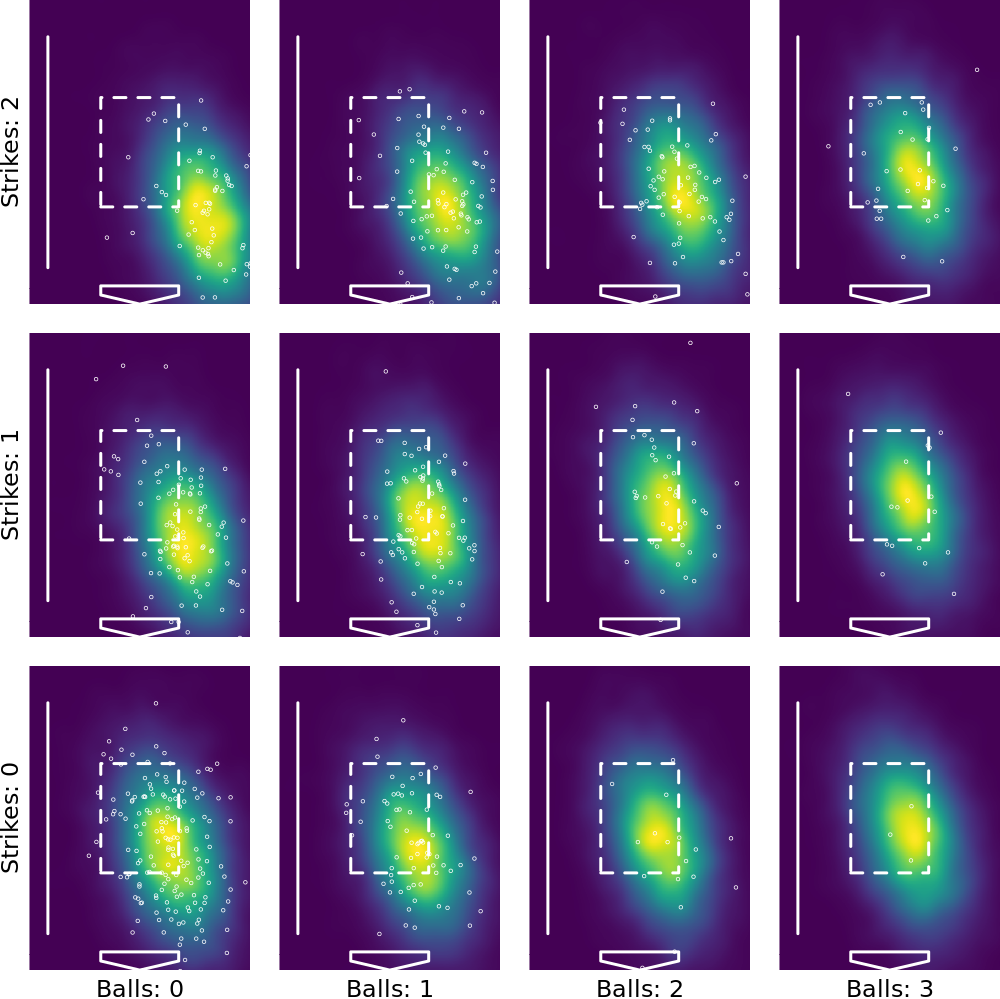
\includegraphics[height = 0.85\textheight]{images/656302_SL_R_plate.png}
  \end{frame}

  \begin{frame}{Does It Work?}
    \centering
    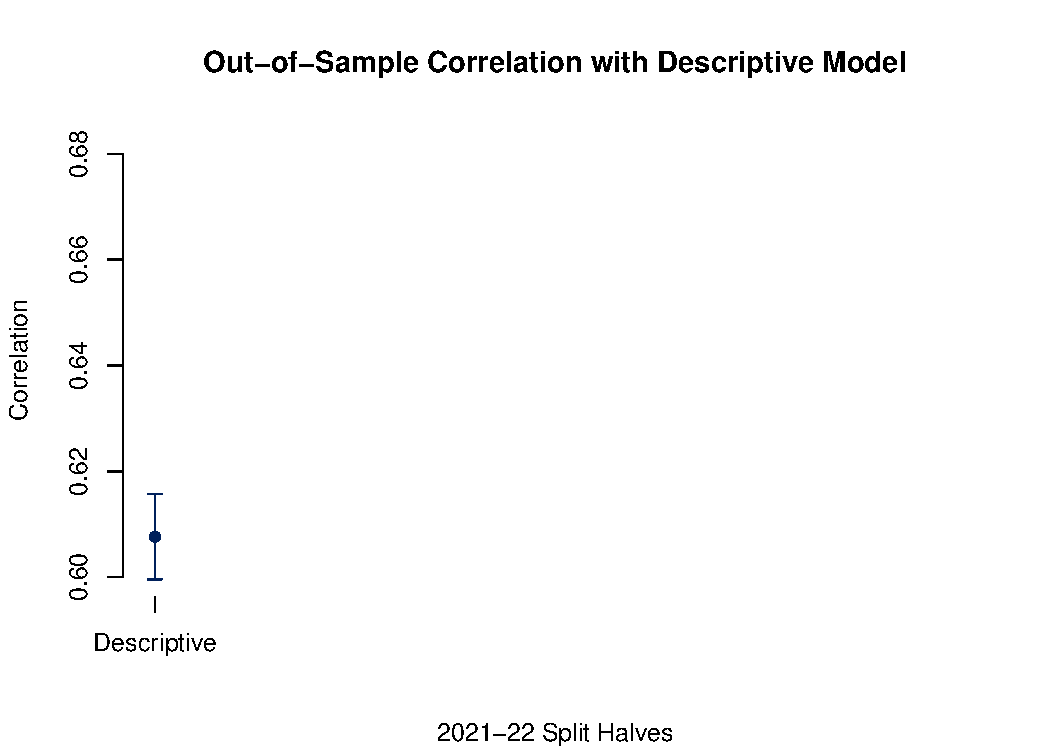
\includegraphics[width = \textwidth]{images/cor_overall_1.pdf}
  \end{frame}

  \begin{frame}{Does It Work?}
    \centering
    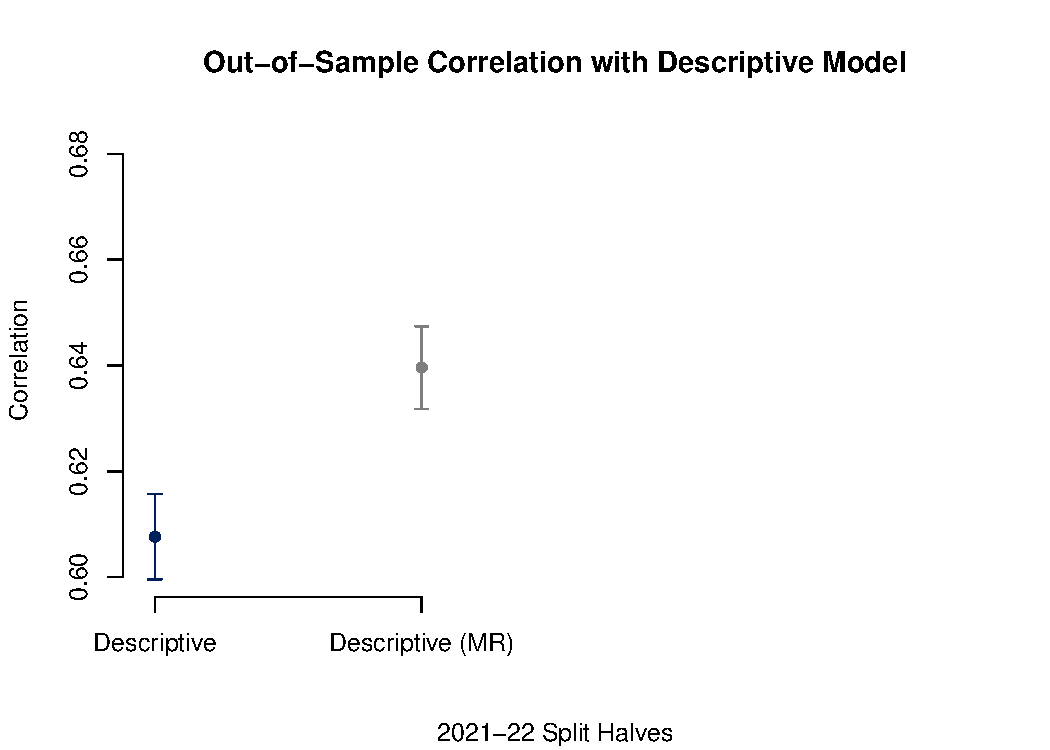
\includegraphics[width = \textwidth]{images/cor_overall_2.pdf}
  \end{frame}

  \begin{frame}{Does It Work?}
    \centering
    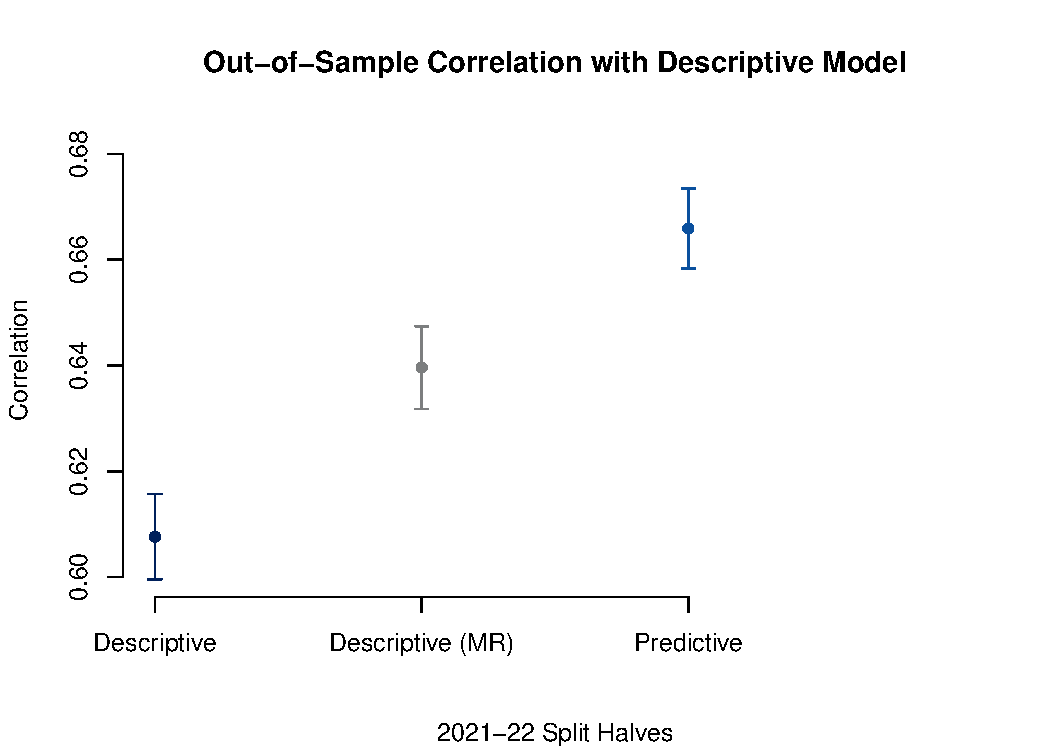
\includegraphics[width = \textwidth]{images/cor_overall_3.pdf}
  \end{frame}

  \begin{frame}{Does It Work?}
    \centering
    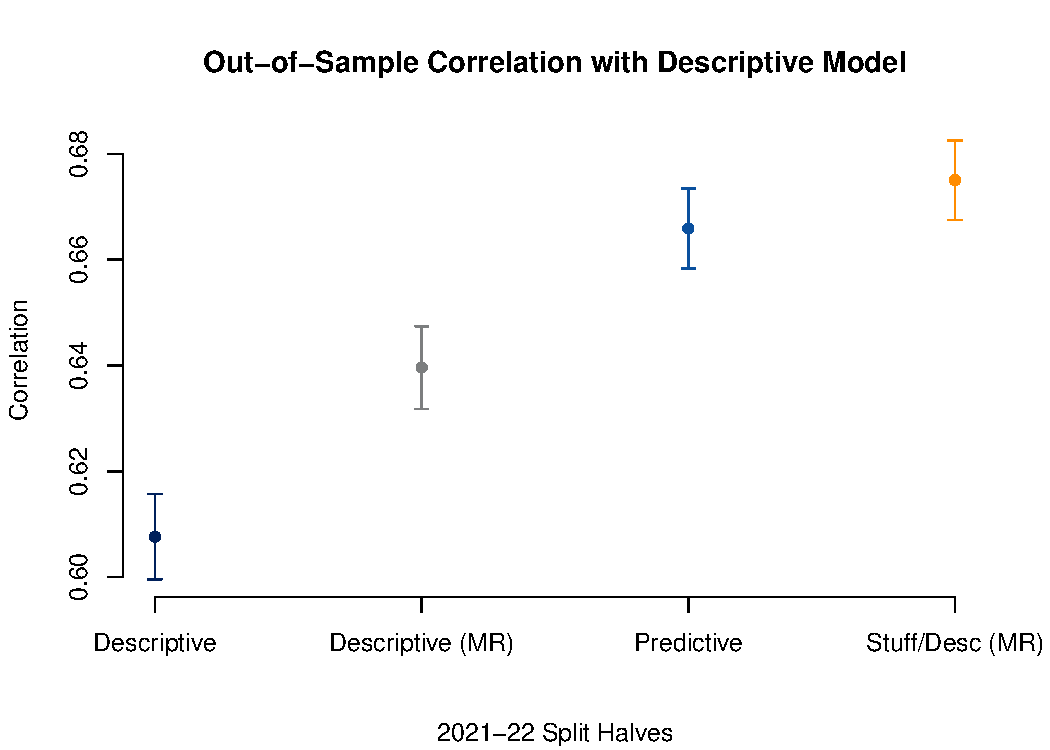
\includegraphics[width = \textwidth]{images/cor_overall_4.pdf}
  \end{frame}
 
  \begin{frame}{Does It Work?}
    \centering
    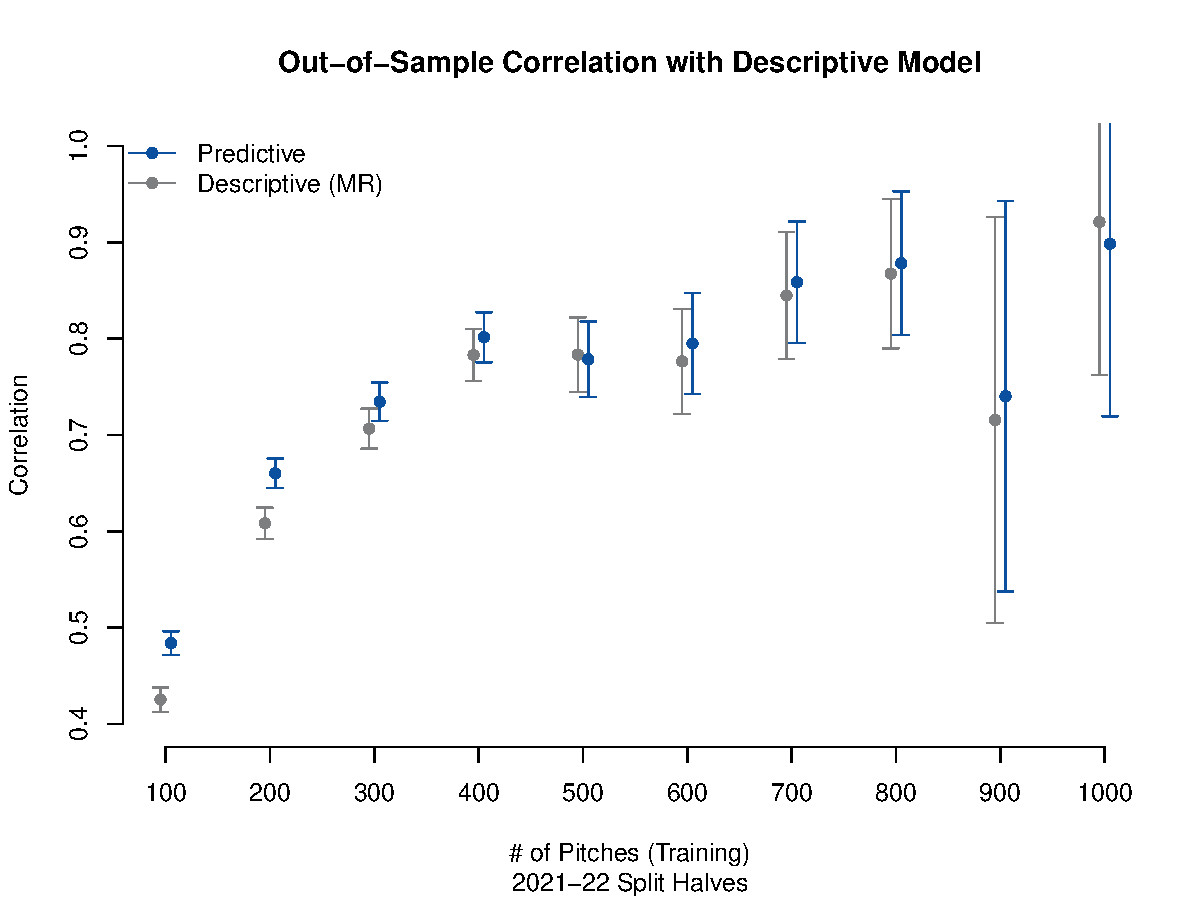
\includegraphics[width = \textwidth]{images/cor_by_sample_size.pdf}
  \end{frame}
 
  \begin{frame}{Leaderboard}
    \centering
    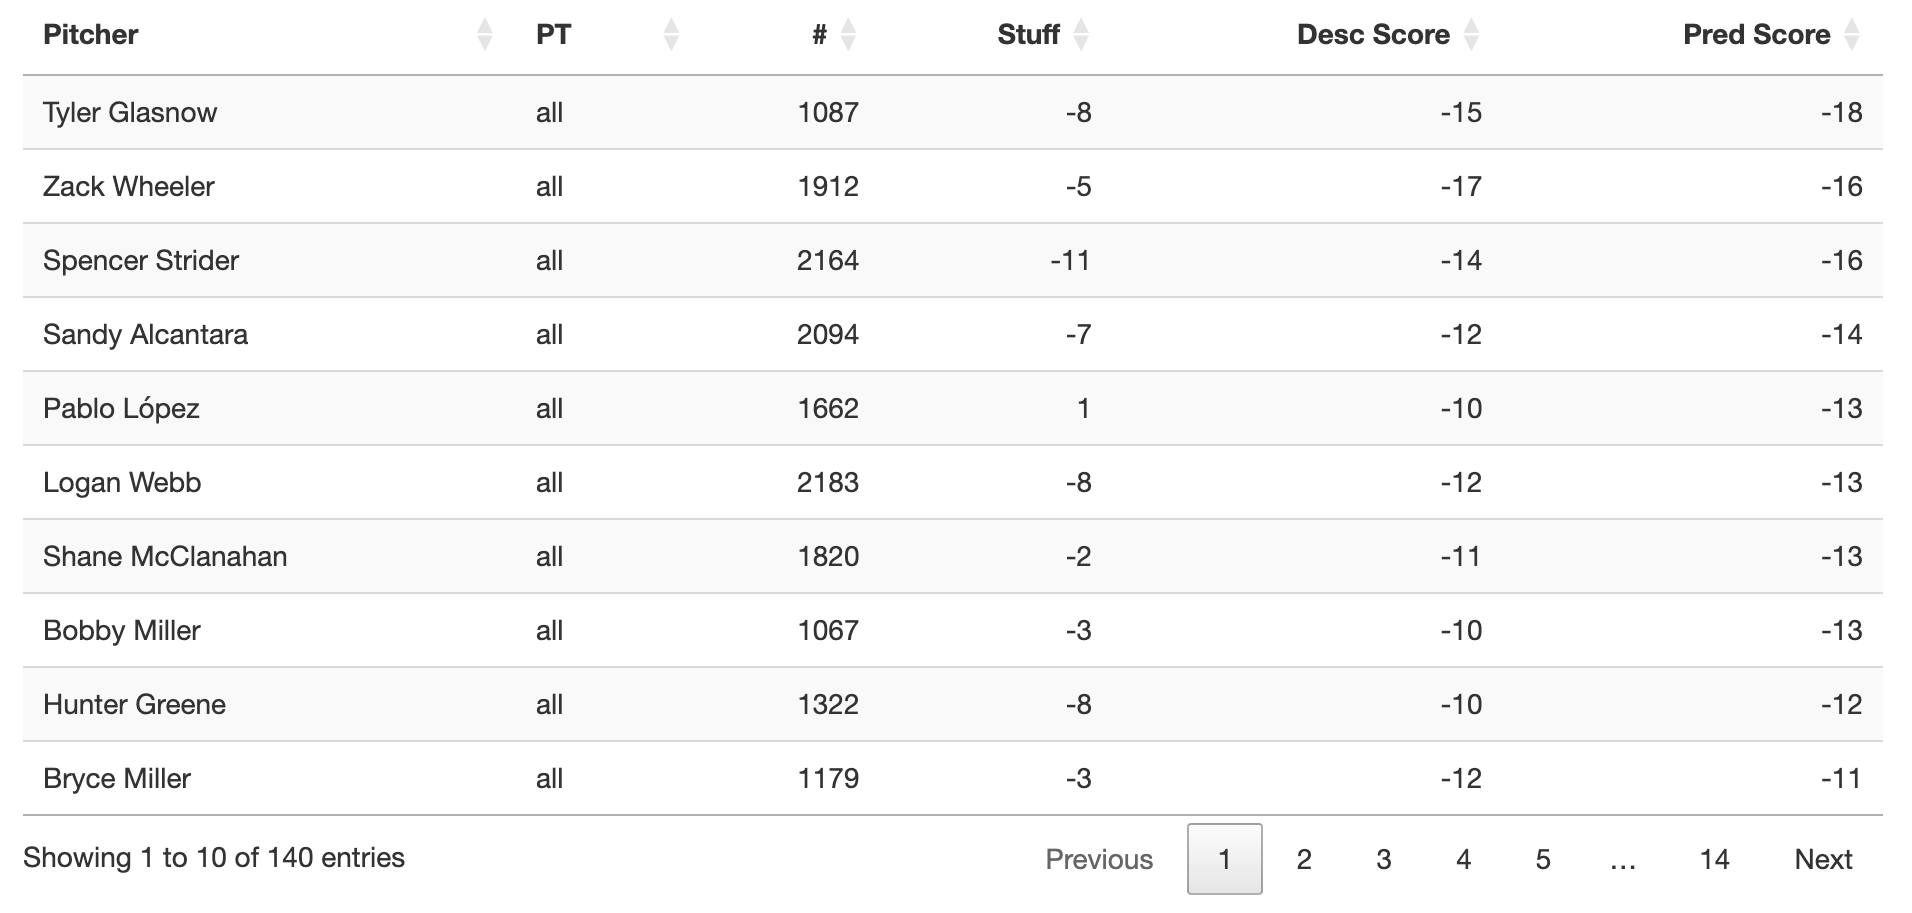
\includegraphics[width = \textwidth]{images/leaderboard.png}
    \vfill
    \centering \scriptsize {\color{ricerichblue}saberpowers}{\color{ricegray}.shinyapps.io/}{\color{ricerichblue}predictive-pitch-score}\\
  \end{frame}

  \begin{frame}{Conclusions}
    Takeaways:
    \begin{enumerate}
      \item Think more about the second source of noise\\
        (random variation in the pitch trajectory itself)
      \item Pitch modeling predictions don't capture\\
        {\it all} of the predictive information in a pitch
    \end{enumerate}
    ~\\
    What's coming up next:
    \begin{itemize}
      \item Better (simpler?) parameterization for distribution model
      \item Relax Gaussian assumption (unimodal with specific tails)
    \end{itemize}
  \end{frame}

  \begin{frame}{Where to Find Us}

    {\color{ricerichblue}saberpowers}{\color{ricegray}.shinyapps.io/}{\color{ricerichblue}predictive-pitch-score}\\
    {\color{ricegray} github.com/}{\color{ricerichblue}saberpowers/predictive-pitch-score}\\
    ~\\
    {\color{ricegray} linkedin.com/in/}{\color{ricerichblue}saberpowers}\\
    {\color{ricegray} twitter.com/}{\color{ricerichblue}saberpowers}\\
    ~\\
    {\color{ricegray} twitter.com/}{\color{ricerichblue}fiftycente1}
  \end{frame}

\end{document}
